\documentclass[11pt]{article}

\usepackage{fix-cm}
\usepackage{tikz}
\usetikzlibrary{shapes,backgrounds,calc,patterns}
\usepackage{amsmath,amsthm} 
\usepackage{mathtools}
\usepackage{amssymb}
\usepackage[framemethod=tikz]{mdframed}
% \usepackage{C:/Users/paulb/VSTeX/local/draculatheme}

\usepackage{mathrsfs}
\usepackage{changepage}
\usepackage{multicol}
\usepackage{hyperref}
\usepackage{slashed}
\usepackage{enumerate}
\usepackage{booktabs}
\usepackage{enumitem}
\usepackage{kantlipsum} 
\usepackage{pgfplots}
\pgfplotsset{compat=1.18}
\usetikzlibrary{decorations.markings}

\setlength{\parindent}{0pt}

\newmdenv[
  topline=false,
  bottomline=true,
  rightline=false,
  leftline=true,
  linewidth=1.5pt,
  linecolor=black, % default color, will be overridden in custom commands
%   backgroundcolor=draculabg, % Needed for Dracula theme
%   fontcolor=draculafg, % Needed for Dracula theme
  innertopmargin=0pt,
  innerbottommargin=5pt,
  innerrightmargin=10pt,
  innerleftmargin=10pt,
  leftmargin=0pt,
  rightmargin=0pt,
  skipabove=\topsep,
  skipbelow=\topsep,
]{customframedproof}

\newenvironment{proofpart}[2][black]{
    \begin{mdframed}[
        topline=false,
        bottomline=false,
        rightline=false,
        leftline=true,
        linewidth=1pt,
        linecolor=#1!40, % Custom color
        % innertopmargin=10pt,
        % innerbottommargin=10pt,
        innerleftmargin=10pt,
        innerrightmargin=10pt,
        leftmargin=0pt,
        rightmargin=0pt,
        % skipabove=\topsep,
        % skipbelow=\topsep%
    ]
    \noindent
    \begin{minipage}[t]{0.08\textwidth}%
        \textbf{#2}%
    \end{minipage}%
    \begin{minipage}[t]{0.90\textwidth}%
        \begin{adjustwidth}{0pt}{0pt}%
}{
    \end{adjustwidth}
    \end{minipage}
    \end{mdframed}
}

\newenvironment{solution}
  {\textit{Solution.}}



%%% AESTHETICS %%%
%-%-%-%-%-%-%-%-%-%-%-%-%-%-%-%-%-%-%-%-%-%-%-%-%-%-%-%-%-%-%-%-%-%-%-%-%-%-%


%%% Dimensions and Spacing %%%
\usepackage[left=0.5in,right=0.5in,top=1in,bottom=1in]{geometry}
% \usepackage{setspace}
% \linespread{1}
\usepackage{listings}
\usepackage{minted}

%%% Define new colors %%%
\usepackage{xcolor}
\definecolor{orangehdx}{rgb}{0.96, 0.51, 0.16}

% Normal colors
\definecolor{xred}{HTML}{BD4242}
\definecolor{xblue}{HTML}{4268BD}
\definecolor{xgreen}{HTML}{52B256}
\definecolor{xpurple}{HTML}{7F52B2}
\definecolor{xorange}{HTML}{FD9337}
\definecolor{xdotted}{HTML}{999999}
\definecolor{xgray}{HTML}{777777}
\definecolor{xcyan}{HTML}{80F5DC}
\definecolor{xpink}{HTML}{F690EA}
\definecolor{xgrayblue}{HTML}{49B095}
\definecolor{xgraycyan}{HTML}{5AA1B9}

% Dark colors
\colorlet{xdarkred}{red!85!black}
\colorlet{xdarkblue}{xblue!85!black}
\colorlet{xdarkgreen}{xgreen!85!black}
\colorlet{xdarkpurple}{xpurple!85!black}
\colorlet{xdarkorange}{xorange!85!black}
\definecolor{xdarkcyan}{HTML}{008B8B}
\colorlet{xdarkgray}{xgray!85!black}

% Very dark colors
\colorlet{xverydarkblue}{xblue!50!black}

% Document-specific colors
\colorlet{normaltextcolor}{black}
\colorlet{figtextcolor}{xblue}

% Enumerated colors
\colorlet{xcol0}{black}
\colorlet{xcol1}{xred}
\colorlet{xcol2}{xblue}
\colorlet{xcol3}{xgreen}
\colorlet{xcol4}{xpurple}
\colorlet{xcol5}{xorange}
\colorlet{xcol6}{xcyan}
\colorlet{xcol7}{xpink!75!black}

% Blue-Purple (should just used colorbrewer...)
\definecolor{xrainbow0}{HTML}{e41a1c}
\definecolor{xrainbow1}{HTML}{a24057}
\definecolor{xrainbow2}{HTML}{606692}
\definecolor{xrainbow3}{HTML}{3a85a8}
\definecolor{xrainbow4}{HTML}{42977e}
\definecolor{xrainbow5}{HTML}{4aaa54}
\definecolor{xrainbow6}{HTML}{629363}
\definecolor{xrainbow7}{HTML}{7e6e85}
\definecolor{xrainbow8}{HTML}{9c509b}
\definecolor{xrainbow9}{HTML}{c4625d}
\definecolor{xrainbow10}{HTML}{eb751f}
\definecolor{xrainbow11}{HTML}{ff9709}

%%% FIGURES %%%
\usepackage{graphicx}  
\graphicspath{ {images/} }  
% \numberwithin{figure}{section}
\usepackage{float}
\usepackage{caption}

%%% Hyperlinks %%%
\usepackage{hyperref}
\definecolor{horange}{HTML}{f58026}
\hypersetup{
	colorlinks=true,
	linkcolor=horange,
	filecolor=horange,      
	urlcolor=horange,
}

\newcommand{\mysqrt}[1]{%
  \mathpalette\foo{#1}%
}
\newcommand{\dmysqrt}[1]{%
  \mathpalette\foodisplay{#1}%
}

\newcommand{\sol}[1]{
    \begin{customframedproof}[linecolor=orangehdx!75,]
        \begin{solution}
        #1
        \end{solution}
    \end{customframedproof}
}

% !TeX spellcheck = off
\newcommand{\foo}[2]{%
  % #1: math style, #2: content
  \sbox0{$#1\sqrt{#2}$}% Measure the size of the standard sqrt in the current style
  \begin{tikzpicture}[baseline=(sqrt.base)]
    \node[inner sep=0, outer sep=0] (sqrt) {$#1\sqrt{#2}$}; % Use the current math style
    \draw([yshift=-0.045em]sqrt.north east) -- ++(0,-0.5ex); % Draw the tick
  \end{tikzpicture}%
}
% !TeX spellcheck = off
\newcommand{\foodisplay}[2]{%
  % #1: math style, #2: content
  \sbox0{$#1\sqrt{#2}$}% Measure the size of the standard sqrt in the current style
  \begin{tikzpicture}[baseline=(sqrt.base)]
    \node[inner sep=0, outer sep=0] (sqrt) {$\displaystyle\sqrt{#2}$}; % Force displaystyle
    \draw[line width=0.4pt] ([yshift=-0.044em]sqrt.north east) -- ++(0,-0.5ex); % Draw the tick
  \end{tikzpicture}%
}

\newcommand{\barNotationT}[1]{\bigg|_{t = #1}}

\newcommand{\cyanit}[1]{\textit{\textcolor{cyan}{#1}}}

\newcommand{\brackett}[1]{\left\langle #1 \right\rangle}

\newcommand{\norm}[1]{\left\lVert \mathbf{#1}\right\rVert}

\newcommand{\proj}{\text{proj}}

\newcommand{\mb}[1]{\mathbf{#1}}

% \renewcommand{\theenumi}{\arabic{enumi}} 
% \renewcommand{\labelenumi}{\theenumi.}

\title{Multivariable Calculus Practice Set I}
\author{Paul Beggs}
\date{\today}

%%% Custom Comands %%%
% Natural Numbers 
\newcommand{\N}{\ensuremath{\mathbb{N}}}

% Whole Numbers
\newcommand{\W}{\ensuremath{\mathbb{W}}}

% Integers
\newcommand{\Z}{\ensuremath{\mathbb{Z}}}

% Rational Numbers
\newcommand{\Q}{\ensuremath{\mathbb{Q}}}

% Real Numbers
\newcommand{\R}{\ensuremath{\mathbb{R}}}

% Complex Numbers
\newcommand{\C}{\ensuremath{\mathbb{C}}}

\newcommand{\I}{\ensuremath{\mathbb{I}}}


\begin{document}

\maketitle

\begin{enumerate}
    \item Consider the curve defined by the parametric equations \(x(t) = \sin(2t)\), \(y(t) = \cos(t)\), for \(0 \leq t \leq 2\pi\).
          \begin{enumerate}
              \item (1 point) Use GeoGebra to graph this curve. Then, plot what you see here, including a well-labeled start and stop and arrows to indicate the trajectory. \\

                    \sol{
                        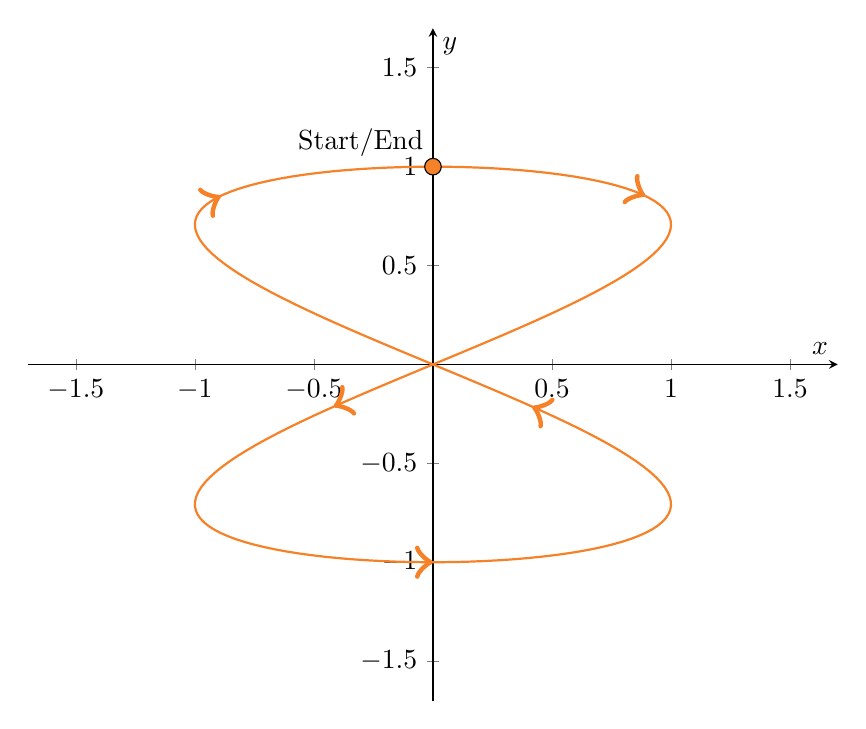
\begin{tikzpicture}
                            \centering
                            \begin{axis}[
                                    xlabel = $x$,
                                    ylabel = $y$,
                                    scale = 1.5,
                                    axis lines = middle,
                                    xmin = -1.5, xmax = 1.5,
                                    ymin = -1.5, ymax = 1.5,
                                    enlargelimits={abs=0.2},
                                ]
                                % Plot the parametric curve with arrows
                                \addplot [
                                    domain = 0:2*pi,
                                    samples = 200,
                                    orangehdx,
                                    thick,
                                    decoration={
                                            markings,
                                            mark=between positions 0.1 and 0.9 step 0.2 with {\arrow[scale=2.5]{>}},
                                        },
                                    postaction={decorate},
                                ] ({sin(deg(2*x))}, {cos(deg(x))});

                                % Mark the start/end point
                                \addplot [only marks, mark=*, mark size=3pt, mark options={fill=orangehdx}] coordinates {(0,1)};
                                \node[above left] at (axis cs:0,1) {Start/End};
                            \end{axis}
                        \end{tikzpicture}
                    }

              \item (2 points) Determine the exact value of the equation of the tangent line when \(t = \pi / 3\). \\

                    \sol{
                        To get the equation of the tangent line, we need to solve for \(\frac{dy}{dt}\) and \(\frac{dx}{dt}\). Solving for \(\frac{dy}{dt}\):
                        \begin{align*}
                            y(t)          & = \cos t   \\
                            \frac{dy}{dt} & = -\sin t.
                        \end{align*}
                        Then, for \(\frac{dx}{dt}\):
                        \begin{align*}
                            x(t)          & = \sin 2t   \\
                            \frac{dx}{dt} & = 2\cos 2t.
                        \end{align*}
                        Now, we have our slope:
                        \[
                            \frac{dy}{dx} = \frac{dy/dt}{dx/dt} = \frac{-\sin t}{2\cos 2t}.
                        \]
                        Evaluated at \(t = \pi / 3\):
                        \[
                            \frac{-\sin t}{2\cos 2t} = \frac{-\mysqrt{3}/2}{-1} = \frac{\mysqrt{3}}{2}.
                        \]
                        Now that we have our slope, we need our points:
                        \[
                            x(\pi / 3) = \sin(2(\pi / 3)) = \sin(\pi / 3) = \mysqrt{3}/2 \qquad \text{and} \qquad y(\pi / 3) = \cos(\pi / 3) = 1/2.
                        \]
                        Putting it all together, we have:
                        \begin{align*}
                            y & = \frac{\mysqrt{3}}{2}(x - \mysqrt{3}/2) + 1/2      \\
                            y & = \frac{\mysqrt{3}}{2}x - \frac{3}{4} + \frac{1}{2} \\
                            y & = \frac{\mysqrt{3}}{2}x - \frac{1}{4}.
                        \end{align*}
                    }

              \item (2 points) Determine the exact value of the geometric area of the region enclosed by curve define above. (Please notice that this area is certainly positive. You might need to think carefully about how to use symmetry to answer this question.) You may find the trigonometric identity \(\cos(2\theta) = 1 - 2 \sin^{2}(\theta)\) useful. You must work out any integrals completely “by-hand,” showing steps to receive credit for this problem. \\

                    \sol{
                        Our set of parametric equations maps out an hourglass shape that has 4 quadrants: 2 positive and 2 negative. Therefore, if we can map one quadrant and multiply it by 4, we can get the total geometric area for the whole shape. Thus, we can restrict our interval such that \(t \in [0, \pi / 2]\).
                        \begin{align*}
                            4\int_{0}^{\pi / 2} y(t)\frac{dx}{dt} \ dt & = 4\int_{0}^{\pi / 2}\cos t(2\cos 2t) \ dt                                                   \\
                                                                       & = 8\int_{0}^{\pi / 2}\cos t(1 - 2 \sin^{2}t) \ dt                                            \\
                                                                       & = 8\int_{0}^{\pi / 2}\cos t - 2\cos t \sin^{2}t \ dt                                         \\
                                                                       & = 8\left[\int_{0}^{\pi / 2} \cos t \ dt - 2\int_{0}^{\pi / 2} \cos t \sin^{2}t \ dt \right]. \\
                        \end{align*}

                        \begin{center}
                            \textsc{Continued on next page.}
                        \end{center}
                        \newpage
                        Now, we can employ \(u\)-substitution to further simplify the intergrand. Thus, let \(u = \sin t\) such that \(\dfrac{du}{\cos t} = dt\). Hence,
                        \begin{align*}
                            8\left[\int_{0}^{\pi / 2} \cos t \ dt - 2\int_{0}^{\pi / 2} \cos t \sin^{2}t \ dt \right] & = 8\left[\int_{0}^{\pi / 2} \cos t \ dt - 2\int_{0}^{\pi / 2} u^{2} \ du \right] \\
                                                                                                                      & = 8\left[\sin t - \frac{2}{3}\sin^{3}t\right]_{0}^{\pi/2}                        \\
                                                                                                                      & = 8\left[1 - \frac{2}{3}\right]                                                  \\
                                                                                                                      & = \frac{8}{3}.
                        \end{align*}
                    }
              \item (2 points) Set up -- but do not evaluate! -- the integral necessary to determine the arc length for this curve. Then, use your calculator to approximate this integral to 3 decimal places. \\

                    \sol{
                        The integral necessary to determine the arc length would be:
                        \[
                            s = \int_{t_{1}}^{t_{2}} \mysqrt{\left(\frac{dx}{dt}\right)^{2} + \left(\frac{dy}{dt}\right)^{2}} \ dt = \int_{0}^{2\pi} \mysqrt{4\cos^{2}2t + \sin^{2}t} \ dt = \boxed{9.429}
                        \]
                    }

          \end{enumerate}
    \item (1 point each) Let \(\mathbf{v} = 3\mathbf{i} - \mathbf{j}\) and \(\mathbf{w} = 2\mathbf{i} + 4\mathbf{j}\).
          \begin{enumerate}
              \item On the axes provided, draw in both \(\mathbf{v}\) and \(\mathbf{w}\).

                    \sol{
                        \begin{tikzpicture}
                            \begin{axis}[
                                    xlabel = $x$,
                                    ylabel = $y$,
                                    scale = 1.5,
                                    axis lines = middle,
                                    xmin = -5, xmax = 5,
                                    ymin = -5, ymax = 5,
                                    enlargelimits={abs=0.5},
                                    step=1,
                                ]
                                % Plot the vectors
                                \addplot [->, xcol1, thick] coordinates {(0,0) (3,-1)};
                                \addplot [->, xcol2, thick] coordinates {(0,0) (2,4)};
                                \addplot [->, xcol3, thick] coordinates {(0,0) (5,3)};

                                \node[above left] at (axis cs:1.5,2.5) {\(\mb{v}\)};
                                \node[above left] at (axis cs:2,-1.2) {\(\mb{w}\)};
                                \node[above left] at (axis cs:4,2.2) {\(\mb{v} + \mb{w}\)};


                            \end{axis}
                        \end{tikzpicture}
                    }
                    \newpage
              \item Find the value of \(\mathbf{v} + \mathbf{w}\) and draw it on the above axes as well.

                    \sol{
                        \[
                            \mb{v} + \mb{w} = \brackett{3 + 2,-1 + 4} = \brackett{5,3}.
                        \]
                        The graph of \(\mb{v} + \mb{w}\) is pictured above.
                    }
              \item Find \(4\mathbf{v} - 2\mathbf{w}\). (It is not necessary to draw this one.)

                    \sol{
                        \[
                            4\mb{v} - 2\mb{w} = \brackett{12 - 4,-4 - 8} = \brackett{8,-12}.
                        \]
                    }
              \item Find the exact value of \(\norm{v}\).
                    \sol{
                        \[
                            \norm{v} = \mysqrt{3^{2} + (-1)^{2}} = \mysqrt{9 + 1} = \mysqrt{10}.
                        \]
                    }
              \item Find a unit vector which points in the same direction as \(\mathbf{v}\).
                    \sol{
                        \[
                            \frac{\mathbf{v}}{\norm{v}} = \frac{\brackett{3,-1}}{\mysqrt{10}} = \brackett{\frac{3}{\mysqrt{10}}, \frac{-1}{\mysqrt{10}}}.
                        \]
                    }
              \item Suppose that we find scalars \(c\) and \(d\) such that \(c\mathbf{v} + d\mathbf{w} = \mathbf{0}\). Show that \(c = 0\) and \(d = 0\).
                    \sol{
                        \[
                            c\mb{v} + d\mb{w} = \brackett{3c + 2d,-c + 4d} = \brackett{0,0}.
                        \]
                        This implies that \(3c + 2d = 0\) and \(-c + 4d = 0\). Solving the system of equations:
                        \[
                            \begin{bmatrix}
                                3  & 2 & 0 \\
                                -1 & 4 & 0
                            \end{bmatrix}
                            \sim
                            \begin{bmatrix}
                                1 & 0 & 0 \\
                                0 & 1 & 0
                            \end{bmatrix},
                        \]
                        we find that \(c = 0\) and \(d = 0\).
                    }
          \end{enumerate}
          \newpage
    \item (1 point each) Suppose that \(\mathbf{u} = 6\mathbf{i} + 2\mathbf{j} - 5\mathbf{k}\) and \(\mathbf{v} = -4\mathbf{i} + \mathbf{j} - 7\mathbf{k}\).
          \begin{enumerate}
              \item Determine \(\mathbf{u} \cdot \mathbf{v}\).
                    \sol{
                        \[
                            \mathbf{u} \cdot \mathbf{v} = (6)(-4) + (2)(1) + (-5)(-7) = -24 + 2 + 35 = 13.
                        \]
                    }
              \item Determine \(\mathbf{u} \times \mathbf{v}\).
                    \sol{
                    \[
                        \mathbf{u} \times \mathbf{v} = \begin{vmatrix}
                            \mathbf{i} & \mathbf{j} & \mathbf{k} \\
                            6          & 2          & -5         \\
                            -4         & 1          & -7
                        \end{vmatrix} = \brackett{\bigl[2(-7) - (-5)(1)\bigr], \ - \bigl[6(-7) - (-5)(-4)\bigr], \ \bigl[6(1) - 2(-4)\bigr]} = \brackett{-9,62,14}.
                    \]
                    }
              \item What is the angle between \(\mathbf{u}\) and \(\mathbf{v}\)? [An answer, in radians rounded to 3 decimal places, is appropriate here.]
                    \sol{
                        First, we need to find the magnitudes of \(\mathbf{u}\) and \(\mathbf{v}\):
                        \[
                            \norm{u} = \mysqrt{6^{2} + 2^{2} + (-5)^{2}} = \mysqrt{65} \qquad \text{and} \qquad \norm{v} = \mysqrt{(-4)^{2} + 1^{2} + (-7)^{2}} = \mysqrt{66}.
                        \]
                        With the magnitudes, we can find the angle between the two vectors:
                        \[
                            \cos \theta = \frac{\mathbf{u} \cdot \mathbf{v}}{\norm{u}\norm{v}} = \frac{13}{\mysqrt{65}\mysqrt{66}} \approx 0.198.
                        \]
                        Thus, \(\theta \approx \cos^{-1}(0.198) \approx \boxed{1.371}\) radians.
                    }
              \item Find \(\proj_{\mathbf{v}}\mathbf{u}\).
                    \sol{
                        \[
                            \proj_{\mathbf{v}}\mathbf{u} = \frac{\mathbf{u} \cdot \mathbf{v}}{\norm{v}^{2}}\mathbf{v} = \frac{13}{66}\brackett{-4,1,-7} = \brackett{-\frac{26}{33},\frac{13}{66},-\frac{91}{66}}.
                        \]
                    }
          \end{enumerate}
    \item (2 points) Determine a parametric equation for the line \textit{segment} that goes from the point \(P = (6,1,-2)\) to \(Q = (-2, 0, 5)\).
          \sol{
              The parametric equation for the line segment is given by:
              \[
                  f(t) = \begin{cases}
                      x(t) = 6 - 8t \\
                      y(t) = 1 - t  \\
                      z(t) = -2 + 7t
                  \end{cases}\text{for } 0 \leq t \leq 1.
              \]
          }
    \item (2 points) Find a symmetric equation for the line which contains the points \(R = (4,-6,1)\) and \(S = (1,2,3)\).
          \sol{
              The symmetric equation for the line is given by:
              \[
                  \frac{x - 4}{-3} = \frac{y + 6}{8} = \frac{z - 1}{-2}.
              \]
          }
          \newpage
    \item (2 points) Find the general form of an equation of the plane which contain the three points \(P = (3,1,-4)\), \(Q = (-2,0,5)\) and \(R = (4,-6,1)\).
          \sol{
          To find the general form of the equation of the plane, we can use the cross product of two vectors that lie in the plane. Let \(\mathbf{PQ} = \brackett{-2 - 3,0 - 1,5 + 4} = \brackett{-5,-1,9}\) and \(\mathbf{PR} = \brackett{4 - 3, -6 - 1, 1 + 4} = \brackett{1,-7,5}\). Then, the normal vector to the plane is given by
          \[\mathbf{PQ} \times \mathbf{QR} = \begin{vmatrix}
                  \mathbf{i} & \mathbf{j} & \mathbf{k} \\
                  -5         & -1         & 9          \\
                  1          & -7         & 5
              \end{vmatrix} = \brackett{[(-1)(5) - 9(-7)], \ -[(-5)(5) - 9(1)], \ [(-5)(-7) - (-1)(1)]} = \brackett{58,34,36}.
          \]
          Thus, \(\mb{n} = \brackett{50,74,24}\) and we can choose the following points to make the equation of the plane:
          \[
              58(x - 3) + 34(y - 1) + 36(z + 4) = 0.
          \]
          To get the \textbf{general equation} of the line, we will expand and simplify:
          \begin{align*}
              58x - 174 + 34y - 34 + 36z + 144 & = 0  \\
              58x + 34y + 36z - 64             & = 0.
          \end{align*}
          }
    \item (2 points) Find an equation, in symmetric form, of the line of intersection between the planes \(2x + y - z + 4 = 0\) and \(x - y + 3z = 1\).
          \sol{
              To find an equation of the line of intersection, we need to add the plane equations to eliminate \(y\):
              \[
                  \begin{array}{ccccccr}
                      2x & + & y            & - & z  & = & -4 \\
                      x  & - & y            & + & 3z & = & 1  \\[1pt]
                      \noalign{\hrule height 1pt}
                      3x &   & \phantom{3y} & + & 2z & = & -3
                  \end{array}
              \]
              Thus, \(x = -1 - \frac{2}{3}z\). Substitute this equation into the first equation to express \(y\) in terms of \(z\):
              \begin{align*}
                  2x + y - z                   & = -4                \\
                  2(-1 - \frac{2}{3}z) + y - z & = -4                \\
                  -\frac{7}{3}z + y            & = -2                \\
                  y                            & = -2 +\frac{7}{3}z.
              \end{align*}
              With \(x\) and \(y\) in terms of \(z\), we need to define \(z\) in terms of \(t\). Choose parameter \(t\) as \(t = -\frac{1}{3}z\). This gives \(z = -3t\). When we substitute our value \(t\) back into the previous two equations, we see that the parametric equations for the line of intersection are \(x = -1 + 2t\), \(y = -2 - 7t\), and \(z = -3t\). Therefore, the symmetric equations for the line are:
              \[
                  \boxed{\frac{x + 1}{2} = \frac{y + 2}{-7} = \frac{z}{-3}.}
              \]
          }
\end{enumerate}


\end{document}